\section{Einleitung}
Vor allem im 21. Jahrhundert wird Umweltfreundlichkeit immer wichtiger. Immer mehr Menschen fahren deshalb und aus vielen anderen Gründen (Gesundheit, Zeitersparnis, etc…) mit dem Fahrrad \citev{fahrrad_nutzung}. In vielen engen (und immer enger werdenden \citev{ritchie_urbanization_2018}) Großstädten der Welt ist das sichere Lagern von Fahrrädern jedoch schwierig bis unmöglich. Herkömmliche Fahrradständer sind zwar platzeffizient und billig, jedoch nicht sicher \citev{leitfaden_vorarlberg}. Besonders bei teuren E-Bikes traut sich mancher nicht, dieses einfach an einen Pfosten zu sperren. Als Alternative dazu gibt es Rad-Boxen oder unterirdische Garagen, beide Optionen sind aber teurer, eingeschränkt nutzerfreundlich und oft zu weit weg von dem Ort, an dem man hinwill.

\begin{figure}[H]
    \centering
    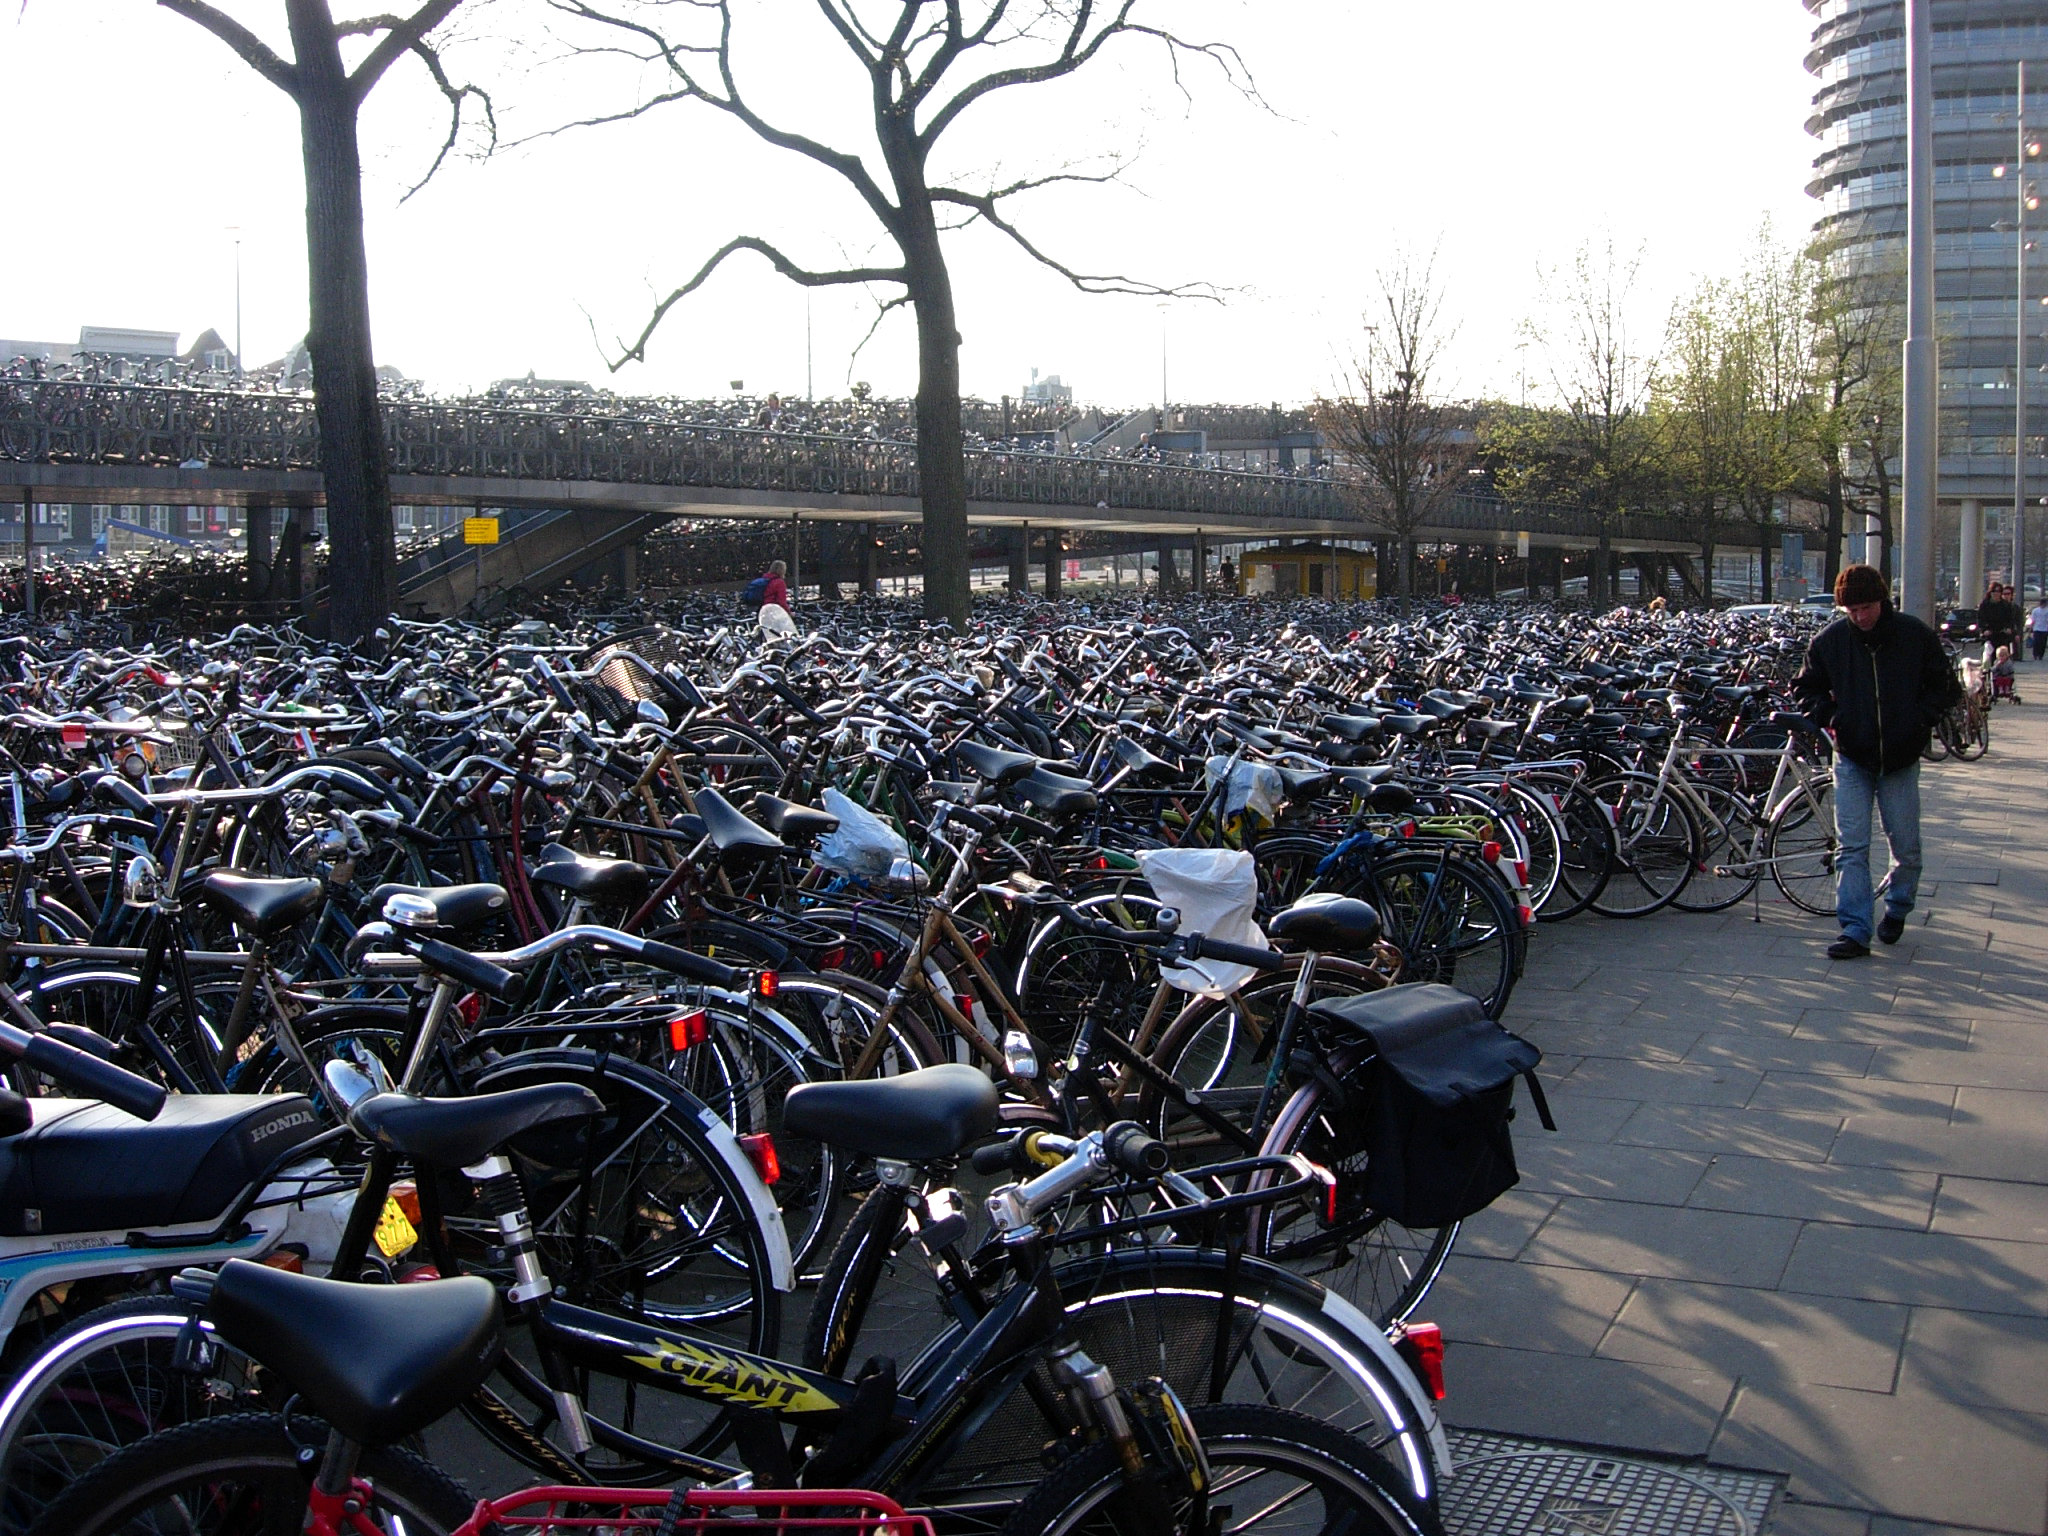
\includegraphics[width=0.45\textwidth]{images/fahrrad_parkhaus_voll}
    \caption{Randvoller Fahrradabstellplatz in Amsterdam \citev{fahrrad_parkhaus_voll}}
    \label{fig:fahrrad_parkhaus_voll}
\end{figure}

In Zukunft wird es sogar noch mehr E-Bikes geben, denn fast die Hälfte aller verkauften Fahrräder sind mit Elektroantrieb ausgestattet (Tendenz stark steigend) \citev{ebike_absatz}. Vor allem der urbane Raum benötigt derzeit dringend Abstellmöglichkeiten, wo Fahrräder schnell, sicher und möglichst billig in der Nähe geparkt werden können.

\clearpage
\subfile{entstehung_der_idee.tex}

\clearpage
\subfile{problemstellung.tex}

\subfile{zielsetzung.tex}
